%%%%%%%%%%%%%%%%%%%%%%%%%%%%%%%%%%%%%%%%%
% Lachaise Assignment
% LaTeX Template
% Version 1.0 (26/6/2018)
%
% This template originates from:
% http://www.LaTeXTemplates.com
%
% Authors:
% Marion Lachaise & François Févotte
% Vel (vel@LaTeXTemplates.com)
%
% License:
% CC BY-NC-SA 3.0 (http://creativecommons.org/licenses/by-nc-sa/3.0/)
% 
%%%%%%%%%%%%%%%%%%%%%%%%%%%%%%%%%%%%%%%%%

%----------------------------------------------------------------------------------------
%	PACKAGES AND OTHER DOCUMENT CONFIGURATIONS
%----------------------------------------------------------------------------------------

\documentclass{article}

%%%%%%%%%%%%%%%%%%%%%%%%%%%%%%%%%%%%%%%%%
% Lachaise Assignment
% Structure Specification File
% Version 1.0 (26/6/2018)
%
% This template originates from:
% http://www.LaTeXTemplates.com
%
% Authors:
% Marion Lachaise & François Févotte
% Vel (vel@LaTeXTemplates.com)
%
% License:
% CC BY-NC-SA 3.0 (http://creativecommons.org/licenses/by-nc-sa/3.0/)
% 
%%%%%%%%%%%%%%%%%%%%%%%%%%%%%%%%%%%%%%%%%

%----------------------------------------------------------------------------------------
%	PACKAGES AND OTHER DOCUMENT CONFIGURATIONS
%----------------------------------------------------------------------------------------

\usepackage{amsmath,amsfonts,stmaryrd,amssymb} % Math packages

\usepackage{enumerate} % Custom item numbers for enumerations

\usepackage[ruled]{algorithm2e} % Algorithms

\usepackage[framemethod=tikz]{mdframed} % Allows defining custom boxed/framed environments

\usepackage{listings} % File listings, with syntax highlighting
\lstset{
	basicstyle=\ttfamily, % Typeset listings in monospace font
}

%----------------------------------------------------------------------------------------
%	DOCUMENT MARGINS
%----------------------------------------------------------------------------------------

\usepackage{geometry} % Required for adjusting page dimensions and margins

\geometry{
	paper=a4paper, % Paper size, change to letterpaper for US letter size
	top=2.5cm, % Top margin
	bottom=3cm, % Bottom margin
	left=2.5cm, % Left margin
	right=2.5cm, % Right margin
	headheight=14pt, % Header height
	footskip=1.5cm, % Space from the bottom margin to the baseline of the footer
	headsep=1.2cm, % Space from the top margin to the baseline of the header
	%showframe, % Uncomment to show how the type block is set on the page
}

%----------------------------------------------------------------------------------------
%	FONTS
%----------------------------------------------------------------------------------------

\usepackage[utf8]{inputenc} % Required for inputting international characters
\usepackage[T1]{fontenc} % Output font encoding for international characters

\usepackage{XCharter} % Use the XCharter fonts

%----------------------------------------------------------------------------------------
%	COMMAND LINE ENVIRONMENT
%----------------------------------------------------------------------------------------

% Usage:
% \begin{commandline}
%	\begin{verbatim}
%		$ ls
%		
%		Applications	Desktop	...
%	\end{verbatim}
% \end{commandline}

\mdfdefinestyle{commandline}{
	leftmargin=10pt,
	rightmargin=10pt,
	innerleftmargin=15pt,
	middlelinecolor=black!50!white,
	middlelinewidth=2pt,
	frametitlerule=false,
	backgroundcolor=black!5!white,
	frametitle={Command Line},
	frametitlefont={\normalfont\sffamily\color{white}\hspace{-1em}},
	frametitlebackgroundcolor=black!50!white,
	nobreak,
}

% Define a custom environment for command-line snapshots
\newenvironment{commandline}{
	\medskip
	\begin{mdframed}[style=commandline]
}{
	\end{mdframed}
	\medskip
}

%----------------------------------------------------------------------------------------
%	FILE CONTENTS ENVIRONMENT
%----------------------------------------------------------------------------------------

% Usage:
% \begin{file}[optional filename, defaults to "File"]
%	File contents, for example, with a listings environment
% \end{file}

\mdfdefinestyle{file}{
	innertopmargin=1.6\baselineskip,
	innerbottommargin=0.8\baselineskip,
	topline=false, bottomline=false,
	leftline=false, rightline=false,
	leftmargin=2cm,
	rightmargin=2cm,
	singleextra={%
		\draw[fill=black!10!white](P)++(0,-1.2em)rectangle(P-|O);
		\node[anchor=north west]
		at(P-|O){\ttfamily\mdfilename};
		%
		\def\l{3em}
		\draw(O-|P)++(-\l,0)--++(\l,\l)--(P)--(P-|O)--(O)--cycle;
		\draw(O-|P)++(-\l,0)--++(0,\l)--++(\l,0);
	},
	nobreak,
}

% Define a custom environment for file contents
\newenvironment{file}[1][File]{ % Set the default filename to "File"
	\medskip
	\newcommand{\mdfilename}{#1}
	\begin{mdframed}[style=file]
}{
	\end{mdframed}
	\medskip
}

%----------------------------------------------------------------------------------------
%	NUMBERED QUESTIONS ENVIRONMENT
%----------------------------------------------------------------------------------------

% Usage:
% \begin{question}[optional title]
%	Question contents
% \end{question}

\mdfdefinestyle{question}{
	innertopmargin=1.2\baselineskip,
	innerbottommargin=0.8\baselineskip,
	roundcorner=5pt,
	nobreak,
	singleextra={%
		\draw(P-|O)node[xshift=1em,anchor=west,fill=white,draw,rounded corners=5pt]{%
		Question \theQuestion\questionTitle};
	},
}

\newcounter{Question} % Stores the current question number that gets iterated with each new question

% Define a custom environment for numbered questions
\newenvironment{question}[1][\unskip]{
	\bigskip
	\stepcounter{Question}
	\newcommand{\questionTitle}{~#1}
	\begin{mdframed}[style=question]
}{
	\end{mdframed}
	\medskip
}

%----------------------------------------------------------------------------------------
%	WARNING TEXT ENVIRONMENT
%----------------------------------------------------------------------------------------

% Usage:
% \begin{warn}[optional title, defaults to "Warning:"]
%	Contents
% \end{warn}

\mdfdefinestyle{warning}{
	topline=false, bottomline=false,
	leftline=false, rightline=false,
	nobreak,
	singleextra={%
		\draw(P-|O)++(-0.5em,0)node(tmp1){};
		\draw(P-|O)++(0.5em,0)node(tmp2){};
		\fill[black,rotate around={45:(P-|O)}](tmp1)rectangle(tmp2);
		\node at(P-|O){\color{white}\scriptsize\bf !};
		\draw[very thick](P-|O)++(0,-1em)--(O);%--(O-|P);
	}
}

% Define a custom environment for warning text
\newenvironment{warn}[1][Warning:]{ % Set the default warning to "Warning:"
	\medskip
	\begin{mdframed}[style=warning]
		\noindent{\textbf{#1}}
}{
	\end{mdframed}
}

%----------------------------------------------------------------------------------------
%	INFORMATION ENVIRONMENT
%----------------------------------------------------------------------------------------

% Usage:
% \begin{info}[optional title, defaults to "Info:"]
% 	contents
% 	\end{info}

\mdfdefinestyle{info}{%
	topline=false, bottomline=false,
	leftline=false, rightline=false,
	nobreak,
	singleextra={%
		\fill[black](P-|O)circle[radius=0.4em];
		\node at(P-|O){\color{white}\scriptsize\bf i};
		\draw[very thick](P-|O)++(0,-0.8em)--(O);%--(O-|P);
	}
}

% Define a custom environment for information
\newenvironment{info}[1][Info:]{ % Set the default title to "Info:"
	\medskip
	\begin{mdframed}[style=info]
		\noindent{\textbf{#1}}
}{
	\end{mdframed}
}


 % Include the file specifying the document structure and custom commands

%----------------------------------------------------------------------------------------
%	ASSIGNMENT INFORMATION
%----------------------------------------------------------------------------------------

\title{Problem Set \#5} % Title of the assignment

\author{Saharnaz Babaei\\ \texttt{saharnaz.babaei@grad.moore.sc.edu}} % Author name and email address

\date{ECON815 --- \today} % University, school and/or department name(s) and a date

%----------------------------------------------------------------------------------------

\begin{document}

\maketitle % Print the title

%----------------------------------------------------------------------------------------
%	INTRODUCTION
%----------------------------------------------------------------------------------------

\section*{Elaboration} % Unnumbered section

In this problem set, I use the data from my own paper (\cite{heydari2016effects}) in which I estimated Markov-Switching model to answer the question how the correlation between oil price and the value added of industry and mine sector of Iran is affected by economic factors. What follows is the implementation of the time series data from estimated correlation between oil price and value added of industry and mine sector in Iran in \cite{heidari2013theeffect} along with the required macroeconomic factors based on the literature.

Figure 1 and 2 show that the relationship between imports and the desired correlation seems to be non-linear. Hence, after assessing a linear estimation between variables of interest, I use a non-linear method to the research question. Results for the first linear model is provided in table 1. Where the model is defined as,

\begin{equation}
CORR_t = \beta_0 + \beta_1 GR_t + \beta_2 P_t + \beta_3 REER_t + \beta_4 POIL_t + \beta_5 IM_t + \epsilon_t
\end{equation}

in which, $CORR$, $GR$, $P$, $REER$, $IM$, and $POIL$ are the dynamic conditional correlation between oil price uncertainty and growth of industry and mine sector in Iran, government expenditures, inflation, real effective exchange rate, total imports and crude oil price respectively.  

\begin{figure}[htbp]
	\begin{center}
		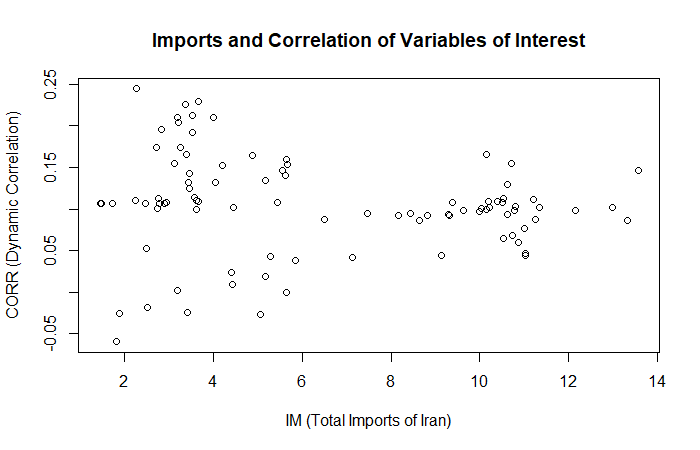
\includegraphics[height=3in]{total_import.png}
		\caption{Relationship between total imports and the dynamic correlation of crude oil price and growth of industry and mine sector in Iran}
	\end{center}
\end{figure}

\begin{figure}[htbp]
	\begin{center}
		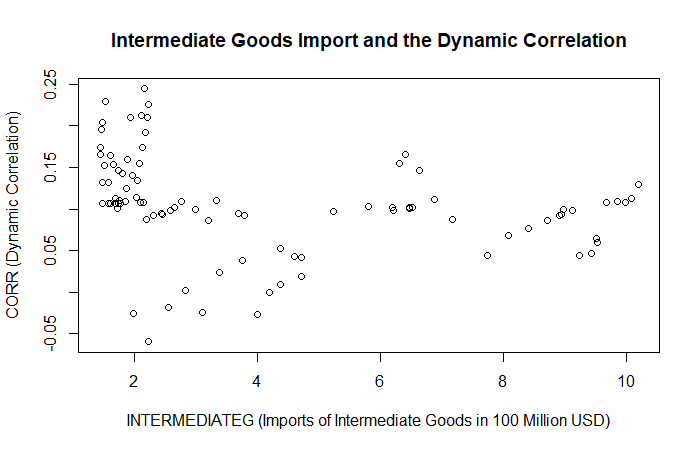
\includegraphics[height=3in]{intermed.png}
		\caption{Relationship between imports of intermediate goods and the estimated dynamic conditional correlation}
	\end{center}
\end{figure}


\begin{figure}[htbp]
	\begin{center}
		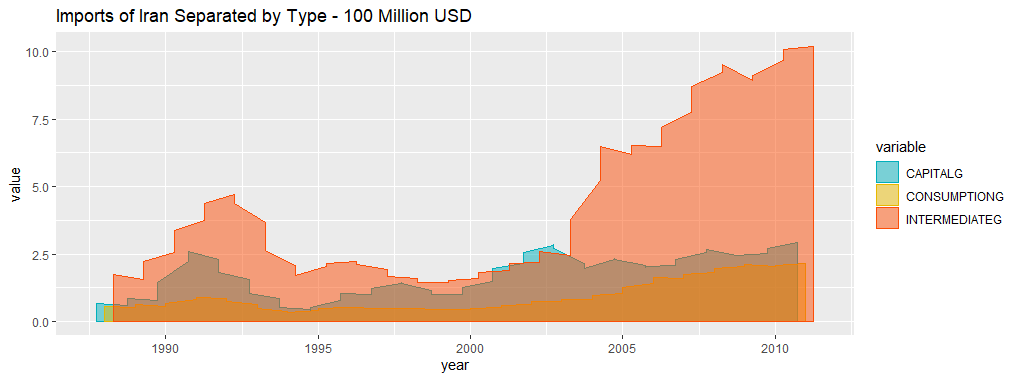
\includegraphics[width=\linewidth]{imports_type.png}
		\caption{Imports separated by the type: import of capital good, consumption goods, and intermediate goods}
	\end{center}
\end{figure}


The second linear specification is to separate the imports to capital goods, consumption goods, and intermediate goods and the model is defined as follows:
\begin{equation}
CORR_t = \beta_0 + \beta_1 GR_t + \beta_2 P_t + \beta_3 REER_t + \beta_4 POIL_t + \beta_5 CAPITALG_t + \beta_6 CONSUMPTIONG_t + \beta_7 INTERMEDIATEG_t + \epsilon_t
\end{equation}

The results for this model are provided in table 2. We can see that 100 billion Rials increase in government expenditures, increases the spillover effect of oil price uncertainty to industry and mine sector by 1.7 percent significantly. One unit increase in the inflation increases the contagion effect by \%23.9 insignificantly. Capital goods and intermediate goods have significant and negative effect on the correlation between oil price and growth of industry and mine sector in Iran which is inconsistent with theory because -- as explained before, imports seem to have a non-linear relationship.  

% latex table generated in R 3.6.1 by xtable 1.8-4 package
% Sun Oct 27 19:53:53 2019
\begin{table}[ht]
	\centering
	\caption{OLS estimation for model 1}
	\begin{tabular}{rrrrr}
		\hline
		& Estimate & Std. Error & t value & Pr($>$$|$t$|$) \\ 
		\hline
		(Intercept) & 0.0889 & 0.0224 & 3.97 & 0.0002 \\ 
		GR & 0.0253 & 0.0062 & 4.08 & 0.0001 \\ 
		P & 0.2533 & 0.1859 & 1.36 & 0.1768 \\ 
		REER & -0.0002 & 0.0001 & -2.55 & 0.0126 \\ 
		POIL & -0.0003 & 0.0004 & -0.71 & 0.4776 \\ 
		IM & -0.0106 & 0.0031 & -3.36 & 0.0012 \\ 
		\hline
	\end{tabular}
\end{table}

% latex table generated in R 3.6.1 by xtable 1.8-4 package
% Sun Oct 27 19:54:12 2019
\begin{table}[ht]
	\centering
	\caption{OLS estimation for model 2}
	\begin{tabular}{rrrrr}
		\hline
		& Estimate & Std. Error & t value & Pr($>$$|$t$|$) \\ 
		\hline
		(Intercept) & 0.1129 & 0.0235 & 4.80 & 0.0000 \\ 
		GR & 0.0173 & 0.0048 & 3.60 & 0.0005 \\ 
		P & 0.2388 & 0.1781 & 1.34 & 0.1836 \\ 
		REER & -0.0002 & 0.0001 & -2.74 & 0.0076 \\ 
		POIL & 0.0004 & 0.0005 & 0.70 & 0.4843 \\ 
		CAPITALG & -0.0287 & 0.0104 & -2.76 & 0.0071 \\ 
		CONSUMPTIONG & 0.0766 & 0.0434 & 1.76 & 0.0817 \\ 
		INTERMEDIATEG & -0.0237 & 0.0078 & -3.05 & 0.0031 \\ 
		\hline
	\end{tabular}
\end{table}


To capture the non-linear relation between the variables of interest, I estimate the Markov-Switching model with two regimes. The results for model 1 and model 2 are provided in table 3 and 4 respectively. The transition probabilities are also provided in these tables indicating that the regimes are stable and they will continue to remain with a probability higher than \%90. Comparing these results with my estimations in my paper, I can say that they are not consistent that can be due to the specification; in the paper, my main equation had a linear part depending on oil price and real effective exchange rate that I could not apply it in R estimations for now. And the non-linear part included government expenditure, inflation, and the imports separated by types. The smoothed probability of the regimes for model 1 and model 2 are provided in figures 4 and 5 respectively. ALL AIC, BIC, and log-likelihood criteria improve in the second model indicating that separating total imports to its ingredients provides a better estimation of parameters. 

\begin{table}
	\centering
	\caption{Markov Switching Model 1}
	\hline
	\verbatiminput{msm1.txt}
	\hline
\end{table}

\begin{table}
	\centering
	\caption{Markov Switching Model 1}
	\hline
	\verbatiminput{msm2.txt}
	\hline
\end{table}

\begin{figure}[htbp]
	\begin{center}
		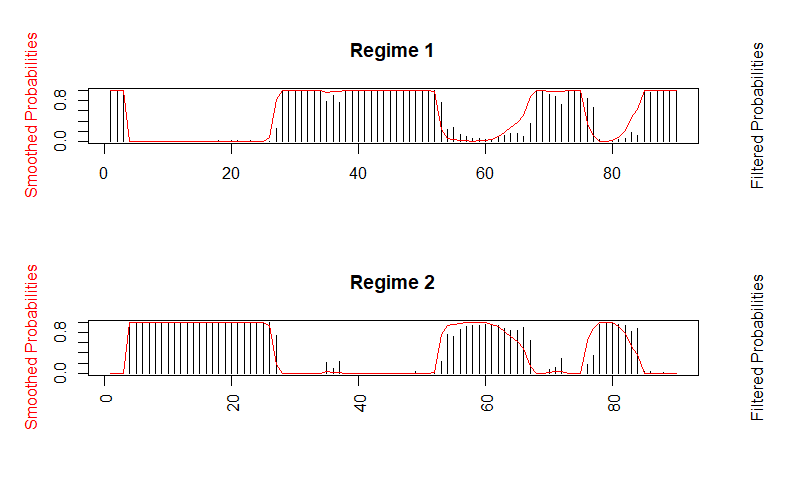
\includegraphics[height=3in]{prob.png}
		\caption{Smoothed transition probabilities for model 1}
	\end{center}
\end{figure}
\begin{figure}[htbp]
	\begin{center}
		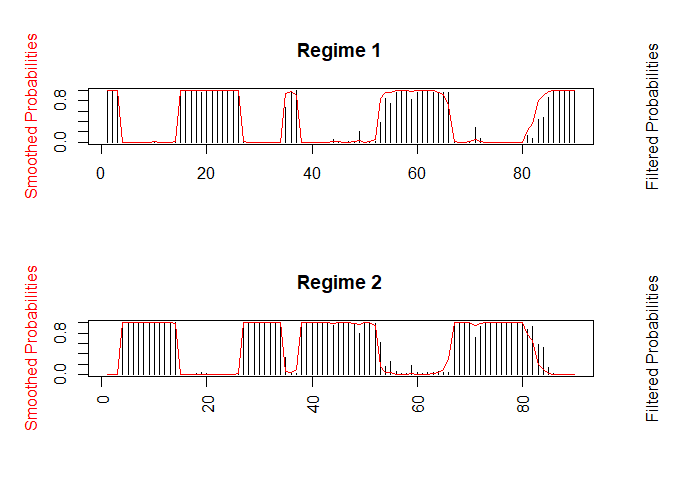
\includegraphics[height=3in]{regimes_model2.png}
		\caption{Smoothed transition probabilities for model 2}
	\end{center}
\end{figure}


%----------------------------------------------------------------------------------------

\bibliographystyle{authordate1}
\bibliography{ref}


\end{document}
